%%%%%%%%%%%%
%
% $Autor: Wings $
% $Datum: 2019-03-05 08:03:15Z $
% $Pfad: Automatisierung/Skript/Produktspezifikation/Powerpoint/AMF.tex $
% $Version: 4250 $
% !TeX spellcheck = en_GB/de_DE
% !TeX encoding = utf8
% !TeX root = filename 
% !TeX TXS-program:bibliography = txs:///biber
%
%%%%%%%%%%%%

\chapter{Project Implementation Steps}

The main focus to implement this project is to train the Arduino Nano 33 BLE Sense for edge computing application. The edge computer will behave and react as the human do after deploying machine learning algorithm and computer vision technique. These are the following outputs we need for completing this project \href{https://www.edgeimpulse.com/}{[Edge Impulse]}.
\begin{itemize}
	\item Gesture Detection
	\item Object Detection
	\item Color Detection
\end{itemize}
Initially I have tried multiple technique to implement the color and object detection part of this project. One of them is Edge Impulse.

\section{Edge Impulse}
Edge Impulse was designed for software developers, engineers and domain experts to solve real problems using machine learning on edge devices without a prior in machine learning. I have tried this platform for color detection, Key word detection, and object detection but later I have switched to other techiques too.Fig\ref{Edge Impulse Flow Chart} shows the different steps involve for training the model.  
\begin{figure}[h]
	\centering
	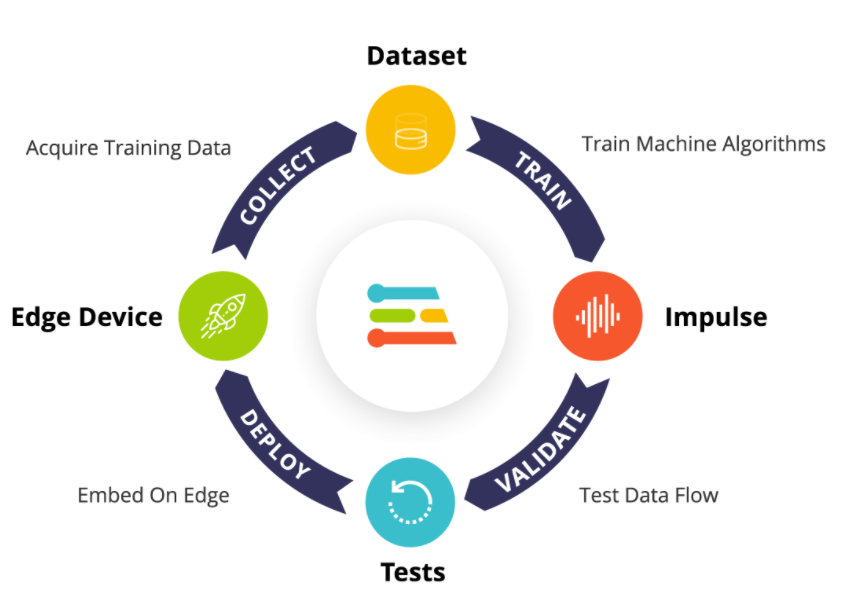
\includegraphics[width=0.6\linewidth]{Nano33BLESense/Edge Impulse}
	\caption{Edge Impulse Flow Chart}
	\label{Edge Impulse Flow Chart}
\end{figure}
Edge impulse can be the great start for beginner, it allow us to make the data set and also assit us during the whole procedure. This platform support particular type of edge computer, Arduino Nano 33 BLE Sense is also one of them.For getting start with edge impulse we need to make a account on edge impulse website. \href{https://www.edgeimpulse.com/}{[Edge Impulse]}.
\begin{itemize}
	\item Edge Impulse is the leading development platform for embedded
	machine learning.
	\item It supports number of embedded hardwares including (Arduin Nano
	33 BLE Sense).
	\item Help us to create data set for Machine learning model.
	\item Shows the uncertainty in data.
	\item Split the data into training (80 percent) and test (20 percent).
	\item Predict the most suitable Machine learning algorithm to train the
	model.
	\item Allow us to test the model and see the accuracy.
	\item After doing all these above steps, we can deploy the train model in
	our Arduino nano 33 BLE Sense
\end{itemize}

\section{Gesture Detection}
Gesture detection is the main task for doing this project. On the basis of different gestures we need to train the Arduino Nano 33 BLE Sense to behave differently on each gesture. My task is cto define the type of gesture what I want to detect, and also recognize these gestures for getting the certain output from Arduino Nano 33 BLE Sense.
\subsection{First Approach for Gesture Detection}
During my research, while going through for defining the type of gestures, I have found very few solutions. One of the most visible solution is the available sensor on Arduino Nano 33 BLE Sense is APDS9960. This sensor can detect four different types of gesture (Moving left, Moving right, Up, Down) these 4 gesture sense the sensor when i move my hand in front of sensor. This was the first solution, and the available library and code is also available in the arduino IDE. I was not satisfy with this solution, because every time the sensor sense the movement when I put my hand very close to the sensor approximately 15mm. So, I switch from sensor detection to Computer vision and Machine learning techniques.
\section{Gesture Detection Test Using MediaPipe}
MediaPipe is the framework in computer vision and support so many Machine learning algorithm to make usefull application. It help us to define to gesture using hand by making the gesture on the basis of hand landmarks. Initially as a test, I have tried to count the finger of hand and show them on the computer using the OpenCV and MediaPipe module. It is detecting very fast and accurate with good frame per second (FPS). Fig\ref{Counting Finger Using MediaPipe and OpenCV} shows the result of counting finger using the MediaPipe technique on the basis of hand landmarks.
\begin{figure}[h]
	\centering
	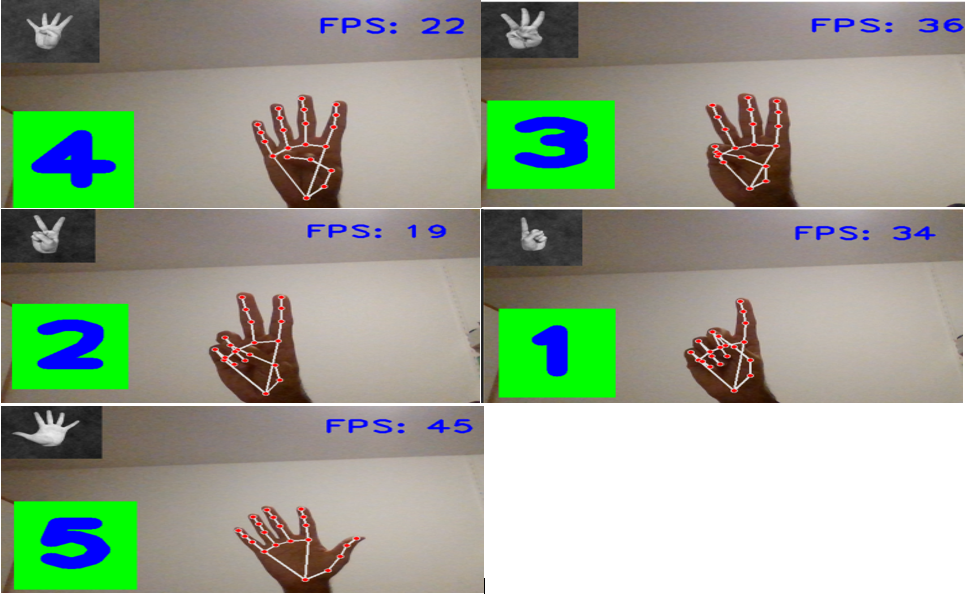
\includegraphics[width=0.5\linewidth]{Nano33BLESense/MediaPipe Check}
	\caption{Counting Finger Using MediaPipe and OpenCV}
	\label{Counting Finger Using MediaPipe and OpenCV}
\end{figure}

\subsection{Successful Approach of Gesture Detection} 
For gesture detection, I choose my hand to define the different types of gesture for edge devices. The most suitable module I found for this is MediaPipe, it help me to make the different types of gesture using the hand landmarks. \href{https://google.github.io/mediapipe/solutions/hands.html}{MediaPipe Hand Landmark Solution} There are 21 hand Landmarks on each hand, we can use the both hand for making the more complex gesture too by changing the position of our fingures or even the individual landmark on hand. Fig\ref{Hand Landmarks using MediaPipe} shows the 21 3D hand landmarks.
\begin{figure}[h]
	\centering
	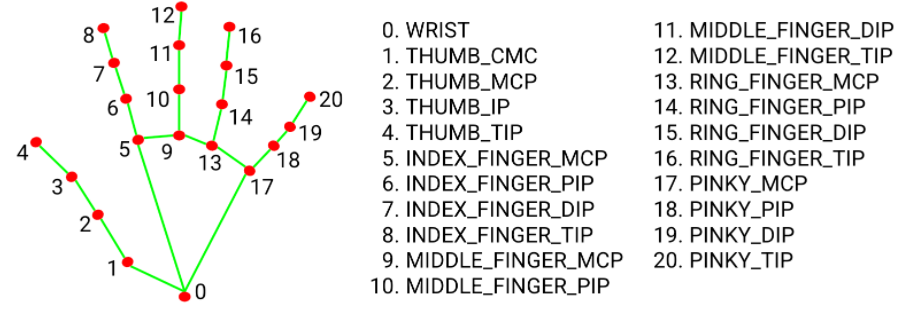
\includegraphics[width=0.6\linewidth]{Nano33BLESense/Hand Landmarks}
	\caption{Hand Landmarks using MediaPipe}
	\label{Hand Landmarks using MediaPipe}
\end{figure}
MediaPipe module uses the convolutional neural network and took 30,000 3D images to train this module. It has very good accuracy and precision, there are some functions written in this module to detect which landmarks we want to detect. Fig\ref{Hand Landmarks using MediaPipe Function} shows for detecting the 21 hand landmarks of the hand are:

\begin{figure}[h]
	\centering
	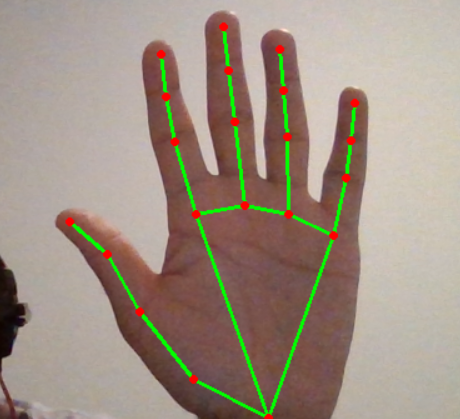
\includegraphics[width=0.7\linewidth]{Nano33BLESense/Landmarks}
	\caption{Hand Landmarks using MediaPipe Function}
	\label{Hand Landmarks using MediaPipe Function}
\end{figure}
With the help of these hand landmarks, we can define the different types of gestures. For example by opening or closing the finger we are able to define and detect gestures or by changing the position of landmarks, by changing position the landmarks also changes the x and y value. MediaPipe help us to detect these changes and also recognize it for getting certain output. The Following two solution I have tried this with the help of MediaPipe Hand Landmarks detection are:
\subsection{Gesture Detection on Arduino Nano 33 BLE Sense}
For doing the Gesture detection on Arduino Nano 33 BLE Sense, I used the following set of Software, framework, Libraries, Modules and Hardwares.
\begin{itemize}
	\item Arduino IDE
	\item Pycharm
	\item Logitech Camera
	\item MediaPipe Algorithm
	\item OpenCV
	\item Pyfirmata
\end{itemize}  
These are the sets of hardware and software pieces I have used for detecting the gestures with Arduino Nano 33 BLE Sense. For the detection part I have define six different outputs on each six different gesture detection. The outputs are (Run, Stop, Slow, Fast, Turn Left, Turn Right). I wrote the Python program in Pycharm software, because MediaPipe module is written in python. Arduino IDE is support only c++, and it is not directly support python libraries and module. Pyfirmata use for seriel communication protocol between python supportive host computer and embedded device have Arduino IDE. By Installing pyfirmata we are able to run the python program on host computer and by serial communication get the results on Arduino Nano 33 BLE Sense. 
Similarly Logitech camera is for capturing the gesture, I have switch to Logitech camera for better resolution and pixels. OpenCV library use for better visualization, writing color function making circles and image processing.
\subsection{Gesture Detection Results On Arduino Nano 33 BLE Sense}
There are six different types of Gestures define and detect by using Hand landmark function of MediaPipe module. The detected signs on the basis of gestures are (Run, Stop, Fast, Slow, Please Turn Left, Please Turn Right). These signs are detect by using the landmarks of hand, and we can define and detect as many gesture by using hand landmark technique. Fig\ref{Gesture Detection on Arduino} shows the detected gestures and sign results are as follow.
\begin{figure}[h]
	\centering
	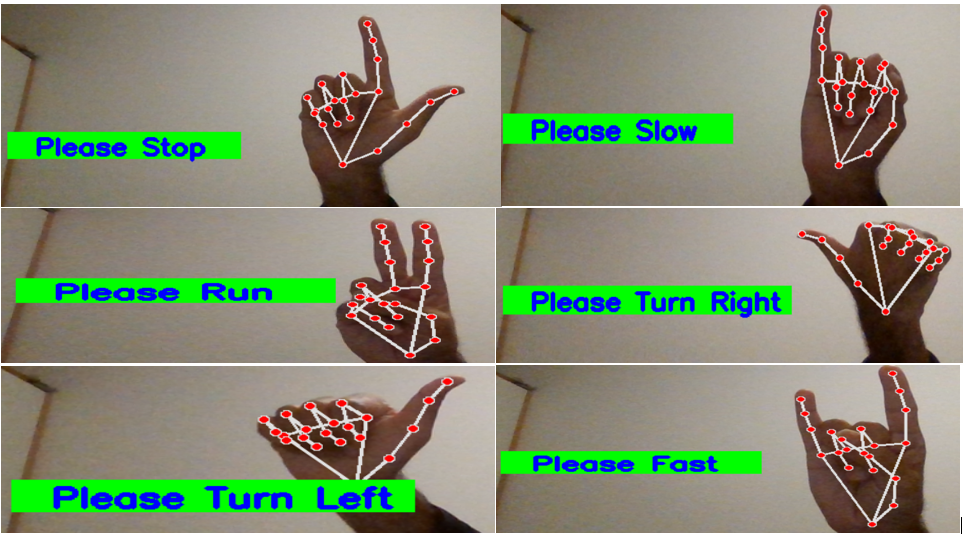
\includegraphics[width=0.7\linewidth]{Nano33BLESense/Arduino Gesture}
	\caption{Gesture Detection on Arduino}
	\label{Gesture Detection on Arduino}
\end{figure}
\section{Gesture Detection Using LSTM Layer and Tensor Flow}
This Model is also equally perform well for detecting the gestures for high processing power computers. The Following sets of Libraries, Software, Module, Hardware, and Packages.
\begin{itemize}
	\item Anaconda (For Jupyter Notebook)
	\item Numpy
	\item Matplotlib
	\item sklearn
	\item TensorFlow 2.6
	\item OpenCV
	\item MediaPipe
	\item CUDA 11.0 
	\item Cudnn 8.2
\end{itemize}
For training the model  I have used the LSTM layer, with Tensorflow for MediaPipe gesture detection. It also detect different types of sign on different gestures. The gestures detect the following five sign (Run, Stop, Slow, Fast, Going Good). I have tried 2000 epochs for training the model but this technique gives the 99 percent accuracy after 300 epochs.
\subsection{Gesture Detection Results Using LSTM and TensorFlow using MediaPipe}
The similar type of gesture detection technique has been tried with long short term memory (LSTM) layer and TensorFlow framework. The model is trained for 5 different classes, (Run, Fast, Slow, Stop, and Going Good(GGood)), these gestures are also detecting using MediaPipe hand Landmarks technique. Fig\ref{Gesture Detection Using LSTM, TensorFlow, and MediaPipe} shows the result of train model detecting the different gestures.
\begin{figure}[h]
	\centering
	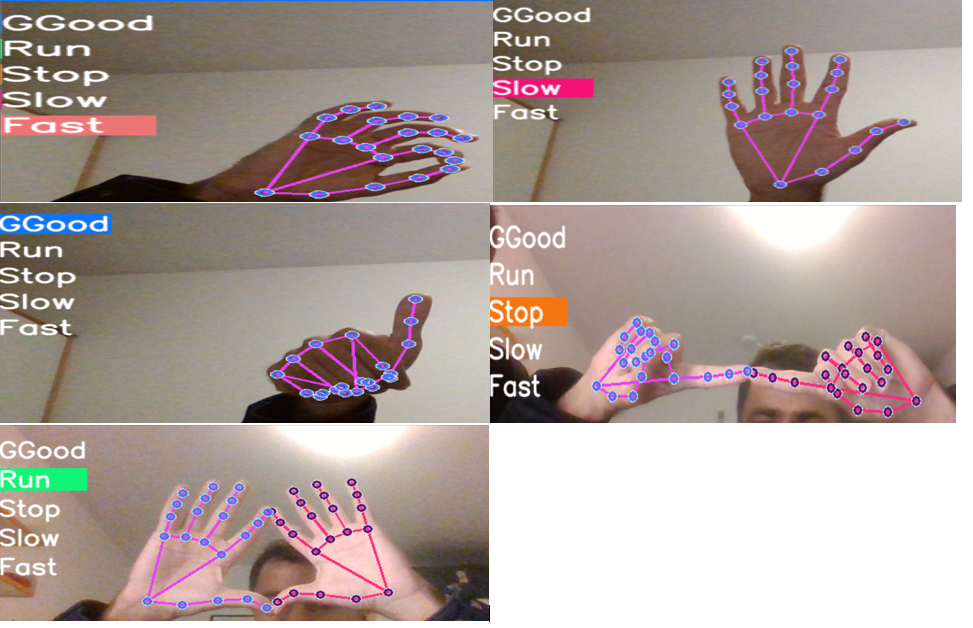
\includegraphics[width=0.7\linewidth]{Nano33BLESense/LSTM Results}
	\caption{Gesture Detection Using LSTM, TensorFlow, and MediaPipe}
	\label{Gesture Detection Using LSTM, TensorFlow, and MediaPipe}
\end{figure}
\section{Color Detection}
For this project, the task is to detect the Red, Green, Blue (RGB) color for different product. In the Arduino Nano 33 BLE Sense, there is on-board sensor APDS9960 whose one of the function is also to detect RGB color. I used this sensor and it give us the RGB percentage of each color in the product. The available program and library is also available in the Arduino IDE for executing this programm.
\section {Object Detection}
There are multiple solution I have tried for object detection too, one with the MediaPipe and other with state of the art object detection models like OpenCV Gpu support using Darknet Yolov4, (You Only Look Once Version 3) Yolov3, (You Only Look Once Version 4) Yolov4, and Deep sort. 
\subsection{Yolov3 and Yolov4 Object Detection Model}
You only look once (YOLO) versions are also performing equally well on COCO data for detecting 80 different classes. YOLO v4 train object detectoin on a single GPU with a smaller mini-batch size. Other models require many GPUs for training with a large mini-batch size, and doing this with one GPU makes the training slow and impractical. The result shows that, YoloV4 has better frame per second (FPS) and Average precision (AP) among others. Fig\ref{Object detection Model Comparison} shows the comparison of YOLO version and other models for object detection is:

\begin{figure}[h]
	\centering
	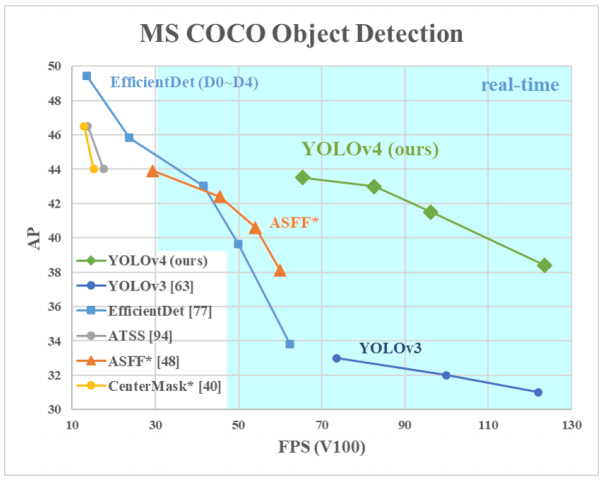
\includegraphics[width=0.7\linewidth]{Nano33BLESense/YOLO}
	\caption{Object detection Model Comparison}
	\label{Object detection Model Comparison}
\end{figure}
\subsection{OpenCV Gpu support using Darknet YOLOV4}
Darknet is an open source neural network framework written in C and CUDA. It is fast, easy to install, and supports CPU and GPU computation. Darknet Yolov4 is the state of the art object detection model, it uses the COCO data set having 80 different classes. It uses the pretrained Yolov4 weigths and able to detect images from photos and videos. The following pre-requisite steps need to follow for setting up the environment:
\begin{itemize}
	\item Install Open-CV from Source with Gpu-support.
	\item Install the CUDA and CUDNN compatible version with open-cv for
	\item Darknet support.
	\item Visual Studio.
	\item Anaconda
\end{itemize}

\subsection{Deep Sort Object Tracking Model}
Deep sort is the model in machine learning use for tracking the object from the video having good frame per second on gpu. It also track 80 different classes and uses COCO data set. It tracks based on not just distance, and velocity but also what that object looks like. Deep sort allows us to add this feature by computing deep features for every bounding box and using the similarity between deep features to also factor into the tracking logic.











\chapter{Open Question and Possible Solution}
It is the time we can say that we have achieve the desired results and implement on Arduino Nano 33 BLE Sense for making the edge computing application. But there are still some checkpoints need to be overview, Although, it is not easy to apply the AI and computer vision both at the same time on such a small and low processing computer.  Instead of low processing power, the Arduino Nano 33 BLE Sense like the other Arduino board supports only Arduino Integrated development environment (IDE) for writing or erasing the code. It is the environment for C++ and not support any python module. The following checkpoints need to be overlook are as follow.


Although, I already get the desire output and results for Arduino Nano 33 BLE Sense. For training the edge computer I used various techniques, all were mentioned in the previous chapters too. There are still some checkpoints (which have alternative solutions available) but we can still work on that more.
\section{Checkpoint 1 (Arduino IDE and Python supportive Packages)}
The Arduino IDE is written only in C++ language and is not supported the other programming languages. Some of the Module I used specially for executing the Gesture detection part of this project is only support python language e.g., MediaPipe and OpenCV. MediaPipe and OpenCV module are the most important part for gesture detection, for detecting the landmarks on hand the supported function is written in python. Without the MediaPipe Module, the hand landmarks technique is not possible to implement. At the moment, there is no such module or library who can support directly MediaPipe Module in Arduino IDE and C++, because MediaPipe Module is written in python. 
\subsection{Possible Solution}
The only possible solution I have found yet is to run the Python Module in Arduino by using the Pyfirmata library available in Arduino environment. Firmata is use as an intermediate protocol that connects an embedded system to a host computer, using pyfirmata the program will run on host computer and get the certain output on embedded Devices.Fig \ref{Python and Arduino} shows the firmata Protocol is use as the communication protocol between the two different environments (C++ and Python). 
\begin{figure}[h]
	\centering
	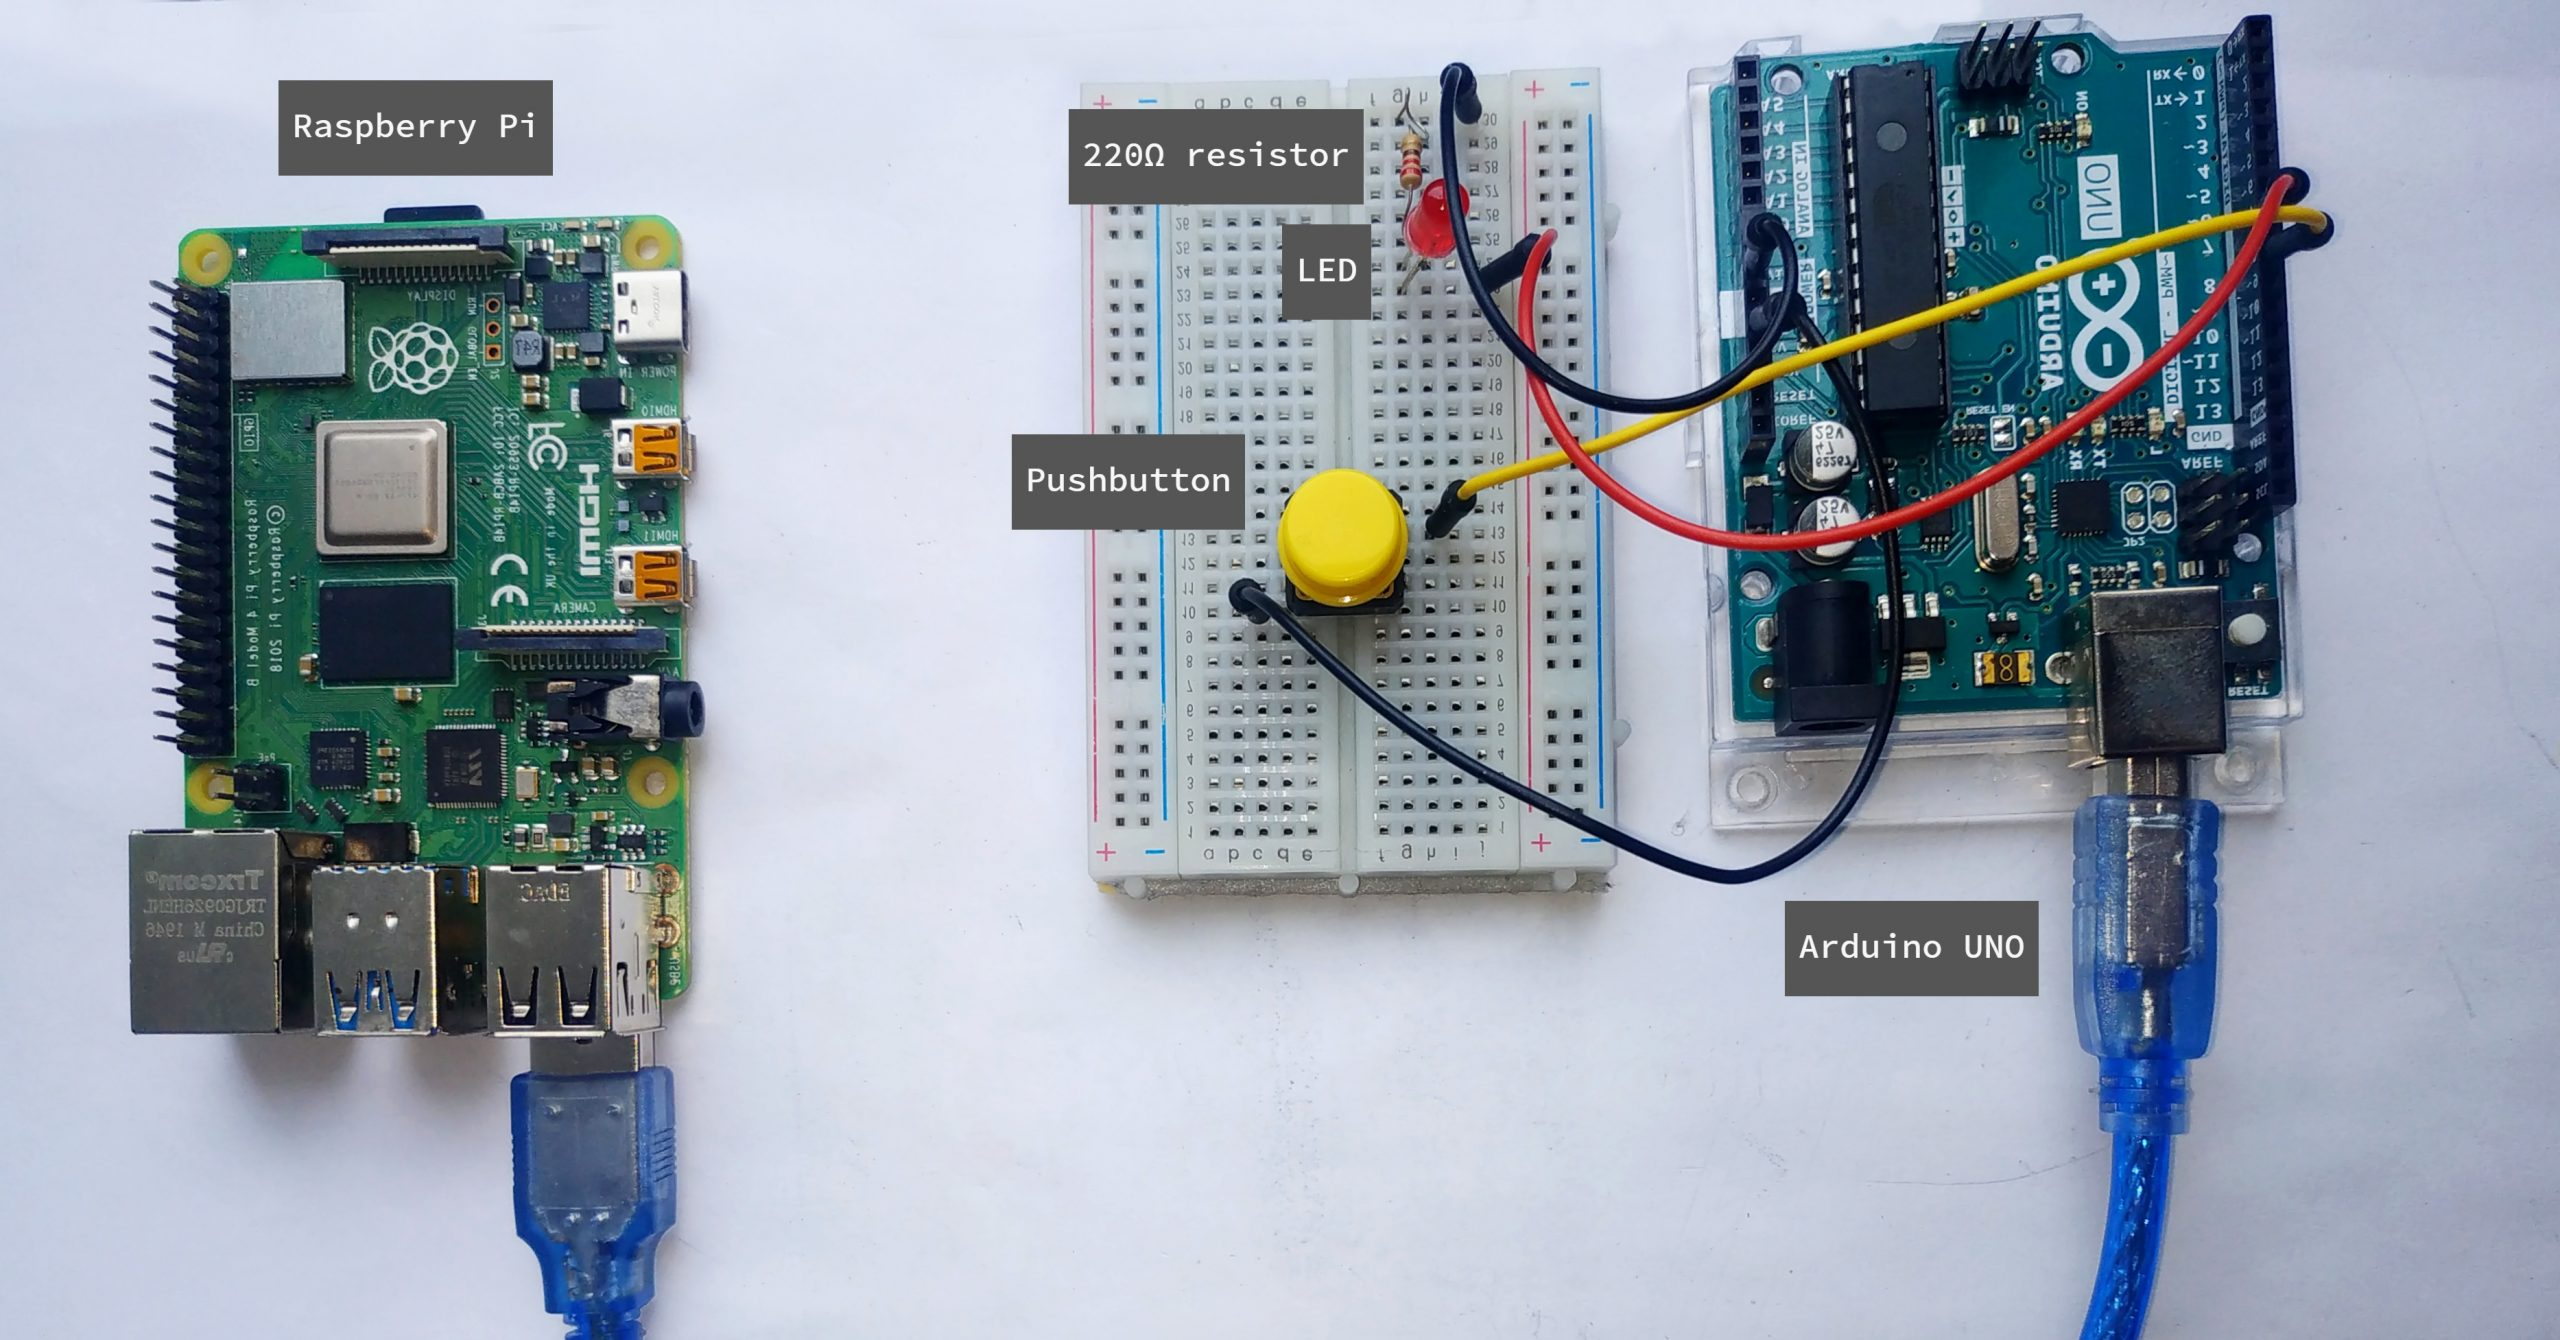
\includegraphics[width=0.7\linewidth]{Nano33BLESense/Pyfirmata}
	\caption{Pyfirmata Communication for Python on Arduino}
	\label{Python and Arduino}
\end{figure}
Initially, the python program needs to run once on any python supported desktop, and by installing the firmata library on Arduino it will make the communication between embedded device and desktop for getting the desire results on Arduino. The Below figure also shows the two environments, the Raspberry pi and Arduino make a communication using firmata protocol. \href{https://roboticsbackend.com/control-arduino-with-python-and-pyfirmata-from-raspberry-pi/}{Arduino and Python}
\section{Checkpoint 2 (Arducam Mini 2MP OV2640 Replacement)}
For getting the high precision and good accuracy, when we are trying to detect some images, we need a high-resolution camera. Nevertheless, the Arducam Mini 2MP is the best suit for Arduino and is most cost effective too, but for better result and accuracy, it is not best suited for the AI and Machine learning application. The main issue with these types of cameras are they need a continue SPI and Cs signal. It has eight pins; all need a continue output from an Arduino Nano 33 BLE Sense at the same time. If any of this damage or loose, the image will not be captured from the Arducam. The other main issue with this camera is that it is not as much accurate for the real time application. For getting the better results we need to come very near to camera every time, it is not suited for any process. There are some of the possible solutions exist, which is easy to implement and making the good results too.
\subsection{Possible solution}
There are many good resolution cameras available for the embedded devices like Arduino Nano 33 BLE Sense, which is easy to use and not as much complicated as the Arducam Mini 2MP is. One of them is (Logitech). It is easy to use, and we can change or displace the camera position very easily.Fig \ref{Logitech Camera} shows the Logitech needs just one Universal Serial Bus (USB) input, and it can operate from desktop or even from any embedded device. The results, reliability, and robustness we have gain by using Logitech camera is much better for machine vision and Artificial Intelligence application. 
\begin{figure}[h]
	\centering
	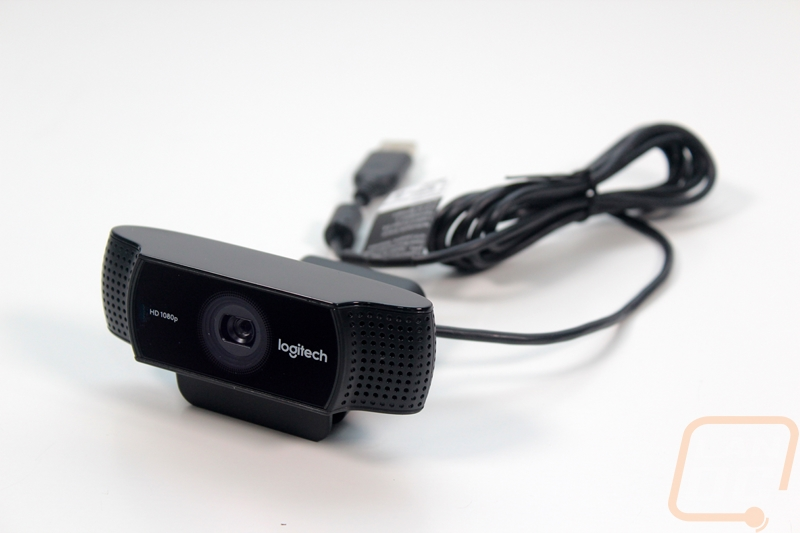
\includegraphics[width=0.7\linewidth]{Nano33BLESense/Logitech}
	\caption{Logitech Camera Replacement}
	\label{Logitech Camera}
\end{figure}
\section{Checkpoint 3 (TensorFlow lite not supported complex object)}
There are still some remaining check points, where we can say that we can apply multiple solutions. There is a possibility to run the already written TensorFlow Lite library in the Arduino IDE for detecting the person detection. It is working equally fine as the other solutions are, but it is only supported the person detection part. We need a Arducam Mini 2MP camera for deploying this Model on Arduino Nano 33 BLE Sense, which has already some limitation because it can detect only when the person is very close to edge computer because edge computer and Arducam must be on the same place all the time due to SPI and CS communication. The other object detection is not possible with TensorFlow lite technique on Arduino Nano 33 BLE Sense due to C++ language environment issues.
\subsection{Possible solution}
Similarly, due to only C++ supported environment, we are not able to run the OpenCV module directly on Arduino IDE. For the person detection, there is a MediaPipe Holistic function called face detection, it can detect the person face with much better accuracy as compared to above mentioned solution. Due to Python supported MediaPipe Module, we can make the communication between python program and Arduino using the Pyfirmata protocol and getting the desired result on Arduino by running the Python and C++ program together. For the image detection we can change the Arducam Mini 2MP with Logitech camera for better and long-distance detection and reduce the complexity. 
\section{Object Detection Part Solution}
For the object detection part other than person, it is not possible directly with Arduino or TensorFlow lite. We need a python supportive module OpenCV, full version of TensorFlow and running some of the state of art object detection Model (Yolo v4, Yolo v3). There are some state of art model for object detection having predefined weights file for detecting 80 different classes are Detectron-2, Deep Sort and Yolo v5. These models need high processing power for detecting the object in random condition, they can detect object as well as track object from the video too. For running these types of models at edge computer we need more Ram, which is impossible on Arduino. These models support OpenCV only when it is installed from the source, which means that for compatibility we need a specific version of TensorFlow and NumPy libraries. 
\section{Possible operating system options for Machine Learning Model}
There is more advancement in this field, either you have to train your model with Central processing unit (CPU) or Graphic processing unit (GPU). Whether for deep learning applications, massive parallelism, intense 3D gaming, or another demanding workload, systems today are being asked to do more than ever before. A central processing unit (CPU) and a graphics processing unit (GPU) have very different roles. In short, the CPU Constructed from millions of transistors, the CPU can have multiple processing cores and is commonly referred to as the brain of the computer, while GPU is a processor that is made up of many smaller and more specialized cores. By working together, the cores deliver massive performance when a processing task can be divided up and processed across many cores. \href{https://www.intel.com/content/www/us/en/products/docs/processors/cpu-vs-gpu.html} {GPU vs CPU}
\subsection{Nvidia GPU Installation requirement}
The Systems having Nvidia GPU capabilities are perform well and quicker when we are trying to train and run the Machine Learning Model as compared to CPU. For running the Model on GPU, we need to install the appropriate version of Computer unified device architecture (CUDA) and cudnn deep neural network library with the OpenCV too. The NVIDIA CUDA® Deep Neural Network library (cuDNN) is a GPU-accelerated library of primitives for deep neural networks. ... It allows them to focus on training neural networks and developing software applications rather than spending time on low-level GPU performance tuning. 

The Arduino support only person detection using the TensorFlow lite, but for the object detection other than person we need a high processing computer and need to install some python module like OpenCV for object detection in random condition.



\chapter{Source Codes}

\subsection{Hand Landmark Tracking}
\begin{verbatim}
	import cv2                            # Import OpenCV Library
	import mediapipe as mp                # Import the MediaPipe Module
	import time                           # Import time Module
	
	cap = cv2.VideoCapture(0)             # Setting up the Webcam
	
	mpHands = mp.solutions.hands          # Use the Hand Landmark function of MediaPipe
	hands = mpHands.Hands()
	mpDraw = mp.solutions.drawing_utils   # For making the connection between Landmarks
	
	pTime = 0                             # (Initialize variables for Frame per second (FPS)
	cTime = 0                             # Current time
	
	while True:                           # Using While Loop for continues detecting 
	success, img = cap.read()             # Read the detecting image
	imgRGB = cv2.cvtColor(img, cv2.COLOR_BGR2RGB) # Convert Color Using OpenCV
	results = hands.process(imgRGB)               # Save the converted Image
	#print(results.multi_hand_landmarks)          # Print the X,Y,Z Value of each landmarks
	
	if results.multi_hand_landmarks:              # Check if there is any detecting hand
	for handLms in results.multi_hand_landmarks:  # When detecting the Landmark
	for id, lm in enumerate(handLms.landmark):    # Handlandmarks according to Id no
	print(id, lm)                                 # Print Handlandmarks as per ID
	h, w, c = img.shape                           # Image shape
	cx, cy = int(lm.x * w), int(lm.y * h)         # Saving the x, and y position of Landmark
	#print(id, cx, cy)                            # Print the X,Y Value of Each Landmark
	
	# if id == 4:                                            # Only For Hand Landmarks # 4 
	cv2.circle(img, (cx, cy), 5, (255, 0, 255), cv2.FILLED)  #Draw circle again each LMS 
	
	mpDraw.draw_landmarks(img, handLms, mpHands.HAND_CONNECTIONS)  # Drawing LMS connection
	
	
	cTime = time.time()         # This is the calculation for Frame per second
	fps = 1 / (cTime - pTime)
	pTime = cTime
	#  Frame Per second calculation end
	cv2.putText(img, str(int(fps)), (10, 70), cv2.FONT_HERSHEY_PLAIN, 3,
	(255, 0, 255), 3)           # Print the FPS for Hand Landmarks detection
	
	cv2.imshow("Image", img)   # For getting the result on desktop
	cv2.waitKey(1)             # Wait for one second
\end{verbatim}


\subsection{Test Example for Counting figure Using Landmark detection}

\begin{verbatim}
	import cv2                            # Import the OpenCV Library
	import time                           # Importing the time
	import os                             # Import os for folder selection
	import HandTrackingModule as htm      # Import the Hand Tracking Module
	
	wCam, hCam = 640, 480                 # Setting the webcam width and heigth
	
	cap = cv2.VideoCapture(0)             # Activate the Webcam for capturing
	cap.set(3, wCam)
	cap.set(4, hCam)
	
	folderPath = "FingerImages"           # File name of save pictures
	myList = os.listdir(folderPath)       # save the directory into variable my list
	print(myList)                         # Print the myList variable
	overlayList = []                      # Initialize the array for saving images
	for imPath in myList:                 # To check which image is detect
	image = cv2.imread(f'{folderPath}/{imPath}')   # Take images from folder a
	#print(f'{folderPath}/{imPath}')
	overlayList.append(image)                      # Appending the image 
	
	print(len(overlayList))                        # Print the total finger 
	
	pTime = 0                                      #  For Per second
	
	detector = htm.handDetector(detectionCon=0.75) # Setting the Detection Threshold
	
	tipIds = [4, 8, 12, 16, 20]                    # Saving the Finger tips Landmarks 
	
	while True:                                      # While Loop for continues capturing
	success, img = cap.read()                        # Read the image is there hand or not
	img = detector.findHands(img)                    # save the detected img
	lmList = detector.findPosition(img, draw=False)  # Seting the lmlist folder
	#print(lmList)                                   # It will show all the LMS
	
	if len(lmList) != 0:        # Check if there is any image available in the list
	fingers = []                # Initialize the empty array
	#if lmList[8][2] < lmList[6][2]: # For specific Case
	#print('Index finger open')      # Index Finger Landmark
	
	# Thumb (This is the code for thumb detection using tipIds)
	if lmList[tipIds[0]][1] > lmList[tipIds[0] - 1][1]:
	fingers.append(1)
	else:
	fingers.append(0)
	# Thumb detection code end
	
	#  Fingers (This is the code for all remaining four fingers)
	for id in range(1, 5):    # For going through all the fingers which one is detected
	if lmList[tipIds[id]][2] < lmList[tipIds[id] - 2][2]:   # Using tipIds of fingers
	fingers.append(1)                                 # Append the finger if it is detected
	else:
	fingers.append(0)                                    # If not detected leave it
	# Finger detection code end
	# print(fingers)   # Print all the fingers
	totalFingers = fingers.count(1)               # Save the detecting finger in variable
	print(totalFingers)                           # Print finger detect on Console
	
	h, w, c = overlayList[totalFingers - 1].shape     # Setting the frame dimension
	img[0:h, 0:w] = overlayList[totalFingers - 1]
	
	# Making the rectangle using OpenCV for Number Counting
	cv2.rectangle(img, (20, 225), (170, 425), (0, 255, 0), cv2.FILLED)
	# Write the text in rectangle using OpenCV
	cv2.putText(img, str(totalFingers), (45, 375), cv2.FONT_HERSHEY_PLAIN,
	10, (255, 0, 0), 25)
	
	# This is the code for Frame Per second (FPS)
	cTime = time.time()
	fps = 1 / (cTime - pTime)
	pTime = cTime
	# Frame per second code end
	
	# This is OpenCV function for showing FPS on the screen, setting color and font size
	cv2.putText(img, f'FPS: {int(fps)}', (400, 70), cv2.FONT_HERSHEY_PLAIN,
	3, (255, 0, 0), 3)
	
	cv2.imshow("Image", img)          # OpenCV function for showing the image
	cv2.waitKey(1)                    # Wait for one second
\end{verbatim}

\subsection{HandTracking Module}
\begin{verbatim}
	import cv2               # Import OpenCV Library
	import mediapipe as mp   # Import MediaPipe Library
	import time              # Import Time
	
	
	class handDetector():        # Make the Hand Detector class for calling in main program
	def __init__(self, mode=False, maxHands=2, detectionCon=0.5, trackCon=0.5):
	self.mode = mode
	self.maxHands = maxHands
	self.detectionCon = detectionCon
	self.trackCon = trackCon
	
	self.mpHands = mp.solutions.hands
	self.hands = self.mpHands.Hands(self.mode, self.maxHands,
	self.detectionCon, self.trackCon)
	self.mpDraw = mp.solutions.drawing_utils
	
	def findHands(self, img, draw=True): # Write the findHands function for detecting hands
	imgRGB = cv2.cvtColor(img, cv2.COLOR_BGR2RGB)
	self.results = self.hands.process(imgRGB)
	# print(results.multi_hand_landmarks)
	
	if self.results.multi_hand_landmarks:
	for handLms in self.results.multi_hand_landmarks:
	if draw:
	self.mpDraw.draw_landmarks(img, handLms,
	self.mpHands.HAND_CONNECTIONS)
	return img
	
	def findPosition(self, img, handNo=0, draw=True): # Finding Position (X,Y) of each LMS
	
	lmList = []
	if self.results.multi_hand_landmarks:
	myHand = self.results.multi_hand_landmarks[handNo]
	for id, lm in enumerate(myHand.landmark):
	# print(id, lm)
	h, w, c = img.shape
	cx, cy = int(lm.x * w), int(lm.y * h)
	# print(id, cx, cy)
	lmList.append([id, cx, cy])
	if draw:
	cv2.circle(img, (cx, cy), 8, (255, 0, 255), cv2.FILLED)
	
	return lmList
	
	
	
	def main():  # Main Function
	pTime = 0
	cTime = 0
	cap = cv2.VideoCapture(0)
	detector = handDetector()
	
	while True:  # For continues detecting
	success, img = cap.read()
	img = detector.findHands(img)
	lmList = detector.findPosition(img)
	if len(lmList) != 0:
	print(lmList[4])
	
	cTime = time.time()        # This is for Frame per second
	fps = 1 / (cTime - pTime) 
	pTime = cTime
	
	cv2.putText(img, str(int(fps)), (10, 70), cv2.FONT_HERSHEY_PLAIN, 3,
	(255, 0, 255), 3)   # For Writing text using OpenCV
	
	cv2.imshow("Image", img)
	cv2.waitKey(1)
	
	
	if __name__ == "__main__":
	main()
	
\end{verbatim}

\subsection{Detecting 6 Different Gesture Code Using Hand Landmarks}
\begin{verbatim}
	import cv2              # Import OpenCV Library
	import mediapipe as mp  # Import MediaPipe Module
	import time             # Import Time
	
	#import controllerad as cnt     # Import the Controllerad module
	
	time.sleep(2.0)                 # Sleep for 2 second
	
	mp_draw = mp.solutions.drawing_utils  # Drawing and Capturing the Hand landmarks
	mp_hand = mp.solutions.hands          # Saving in mp_hand variable
	
	tipIds = [4, 8, 12, 16, 20]  # Use the tip of each finger
	
	video = cv2.VideoCapture(0)  # Activate the Webcam
	
	with mp_hand.Hands(min_detection_confidence=0.9,
	min_tracking_confidence=0.9) as hands:  # Set the detection and tracking confidence
	while True:                # For continues detection
	ret, image = video.read()  # Read the image
	image = cv2.cvtColor(image, cv2.COLOR_BGR2RGB)  # Convert color using OpenCV
	image.flags.writeable = False
	results = hands.process(image)  # Save the results
	image.flags.writeable = True
	image = cv2.cvtColor(image, cv2.COLOR_RGB2BGR)  # Save images in variable
	lmList = []  # Initialize the empty list for image saving
	
	if results.multi_hand_landmarks:  # Check if there is any Hand in the frame or not
	for hand_landmark in results.multi_hand_landmarks:  # Detecting the Landmarks of hand
	myHands = results.multi_hand_landmarks[0]  # Saving the landmarks in variable
	for id, lm in enumerate(myHands.landmark):  # Check all the Ids of fingers
	h, w, c = image.shape  # Saving the image shape as width and height
	cx, cy = int(lm.x * w), int(lm.y * h)  # X, and Y Position
	lmList.append([id, cx, cy])  # Append the X, Y and id of each gesture
	
	mp_draw.draw_landmarks(image, hand_landmark, mp_hand.HAND_CONNECTIONS) # LMS Connection
	fingers = []  # Initialize empty array for saving detection
	
	if len(lmList) != 0:  # Check if there is any hand detection or not
	fingers = []
	
	if (lmList[8][2] < lmList[6][2]) and (
	lmList[20][2] < lmList[18][2]):  # For specific Case When Index and small finger open.
	print('Please Fast')  # Sign will be Please fast for this gesture
	Reaction = 'Fast'  # Save fast in reaction variable
	cv2.rectangle(image, (15, 345), (270, 380), (0, 255, 0), cv2.FILLED)  # Draw rectangle 
	cv2.putText(image, "Please Fast", (45, 375), cv2.FONT_HERSHEY_SIMPLEX,
	1, (255, 0, 0), 3)  # Write text in rectangle
	cnt.led(Reaction) # Getting certain action on Arduino as per the Gesture
	
	elif (lmList[8][2] < lmList[6][2]) and (
	lmList[12][2] < lmList[10][2]):  # For specific Case When Index and middle finger open
	print('Please Run')  # Sign will be Please Run for this gesture
	Reaction = 'Run'  # Save fast in reaction variable
	cv2.rectangle(image, (15, 345), (270, 380), (0, 255, 0), cv2.FILLED)  # Draw rectangle 
	cv2.putText(image, "Please Run", (45, 375), cv2.FONT_HERSHEY_SIMPLEX,
	1, (255, 0, 0), 3)  # Write text in rectangle
	cnt.led(Reaction)   # Getting certain action on Arduino as per the Gesture
	
	elif lmList[20][2] < lmList[18][2]:  # For specific Case When only small finger open
	print('Please Slow')  # Sign will be Please Slow for this gesture
	Reaction = 'Slow'  # Save Slow in reaction variable
	cv2.rectangle(image, (15, 345), (270, 380), (0, 255, 0), cv2.FILLED)  # Draw rectangle 
	cv2.putText(image, "Please Slow", (45, 375), cv2.FONT_HERSHEY_SIMPLEX,
	1, (255, 0, 0), 3)  # Write text in rectangle
	cnt.led(Reaction)  Getting certain action on Arduino as per the Gesture
	
	elif lmList[tipIds[0]][1] > lmList[tipIds[0] - 1][1] and (lmList[8][2] < lmList[6][2]):
	print('please stop')  # Sign will be Please stop for this gesture
	Reaction = 'Stop'  # Save Stop in reaction variable
	cv2.rectangle(image, (15, 345), (270, 380), (0, 255, 0), cv2.FILLED)  # Draw rectangle
	cv2.putText(image, "Please Stop", (45, 375), cv2.FONT_HERSHEY_SIMPLEX,
	1, (255, 0, 0), 3)  # Write text in rectangle
	cnt.led(Reaction) # Getting certain action on Arduino as per the Gesture
	
	elif lmList[tipIds[0]][1] > lmList[tipIds[0] - 1][1]:  # When thumb shows left direction
	print("Please Turn Left")  # Sign will be Please turn left for this gesture
	Reaction = 'Turn Left'  # Save the Turn Left in Reaction variable
	cv2.rectangle(image, (15, 345), (320, 380), (0, 255, 0), cv2.FILLED)  # Draw rectangle 
	cv2.putText(image, "Please Turn Left", (45, 375), cv2.FONT_HERSHEY_SIMPLEX,
	1, (255, 0, 0), 3)  # Write text in rectangle
	cnt.led(Reaction)  # Getting certain action on Arduino as per the Gesture
	
	elif lmList[tipIds[0]][1] < lmList[tipIds[0] - 1][1]: # When thumb shows right direction
	print("Please Turn Right")  # Sign will be Please turn right for this gesture
	Reaction = 'Turn Right'  # Save the Turn right in Reaction variable
	cv2.rectangle(image, (15, 345), (335, 380), (0, 255, 0), cv2.FILLED)  # Draw rectangle 
	cv2.putText(image, "Please Turn Right", (45, 375), cv2.FONT_HERSHEY_SIMPLEX,
	1, (255, 0, 0), 3)  # Write text in rectangle
	cnt.led(Reaction)  # Getting certain action on Arduino as per the Gesture
	
	cv2.imshow("Frame", image)  # Showing the results on desktop
	if cv2.waitKey(10) & 0xFF == ord('q'):  # For smooth quit please press q
	break
	video.release()  # Getting out of programm
	cv2.destroyAllWindows()  # Stop all screen
	
\end{verbatim}

\subsection{Module for Running code on Arduino}
\begin{verbatim}
	import pyfirmata  # Import the Pyfirmata Library
	
	comport = 'COM3'  # Selecting the COM3
	
	board = pyfirmata.Arduino(comport)  # Serial communication with Arduino
	
	led_1 = board.get_pin('d:12:o')  # Initialize Led on Digital pin 12
	led_2 = board.get_pin('d:10:o')  # Initialize Led on Digital pin 10
	led_3 = board.get_pin('d:8:o')   # Initialize Led on Digital pin 8
	led_4 = board.get_pin('d:6:o')   # Initialize Led on Digital pin 6
	led_5 = board.get_pin('d:4:o')   # Initialize Led on Digital pin 4
	led_6 = board.get_pin('d:2:o')   # Initialize Led on Digital pin 2
	
	
	def led(Reaction):  # Writing the Led Function
	if Reaction == 'Run':   # Check the reaction condition
	# Only led_1 turn on, all the others off
	led_1.write(1)      #
	led_2.write(0)
	led_3.write(0)
	led_4.write(0)
	led_5.write(0)
	led_6.write(0)
	elif Reaction == 'Fast':  # Check the reaction condition
	# Only led_2 turn on, all the others off
	led_1.write(0)
	led_2.write(1)
	led_3.write(0)
	led_4.write(0)
	led_5.write(0)
	led_6.write(0)
	elif Reaction == 'Stop':  # Check the reaction condition
	# Only led_1, led_3, led_5 turn on, all the others off
	led_1.write(1)
	led_2.write(0)
	led_3.write(1)
	led_4.write(0)
	led_5.write(1)
	led_6.write(0)
	elif Reaction == 'Slow':  # Check the reaction condition
	# Only led_4 turn on, all the others off
	led_1.write(0)
	led_2.write(0)
	led_3.write(0)
	led_4.write(1)
	led_5.write(0)
	led_6.write(0)
	elif Reaction == 'Turn Left':  # Check the reaction condition
	# Only led_5 turn on, all the others off
	led_1.write(0)
	led_2.write(0)
	led_3.write(0)
	led_4.write(0)
	led_5.write(1)
	led_6.write(0)
	elif Reaction == 'Turn Right':  # Check the reaction condition
	# Only led_6 turn on, all the others off
	led_1.write(0)
	led_2.write(0)
	led_3.write(0)
	led_4.write(0)
	led_5.write(0)
	led_6.write(1)
	
\end{verbatim}
